\subsection{Konstante globale Problemmenge}
In einem ersten Schritt wurde versucht alle Probleme mithilfe einer konstanten, globalen Problemmenge zu lösen. Dabei fiel auf, dass dieser Algorithmus, unabhängig vom Problem, mit sowohl der Grösse der Problemmenge als auch der Populationsgrösse skaliert. Ein gutes Beispiel für dieses Verhalten ist in Abbildung \ref{fig:c_g_div5} dargestellt. Auf der X-Achse sind sowohl die Grösse der Problemmenge (z.B. $P:50$) als auch die Populationsgrösse (z.B. $C:100$) abgebildet. Auf der Y-Achse sieht man die Performance des Algorithmus bei den jeweiligen Eingabeparametern.

\begin{figure}[h]
  \centering
  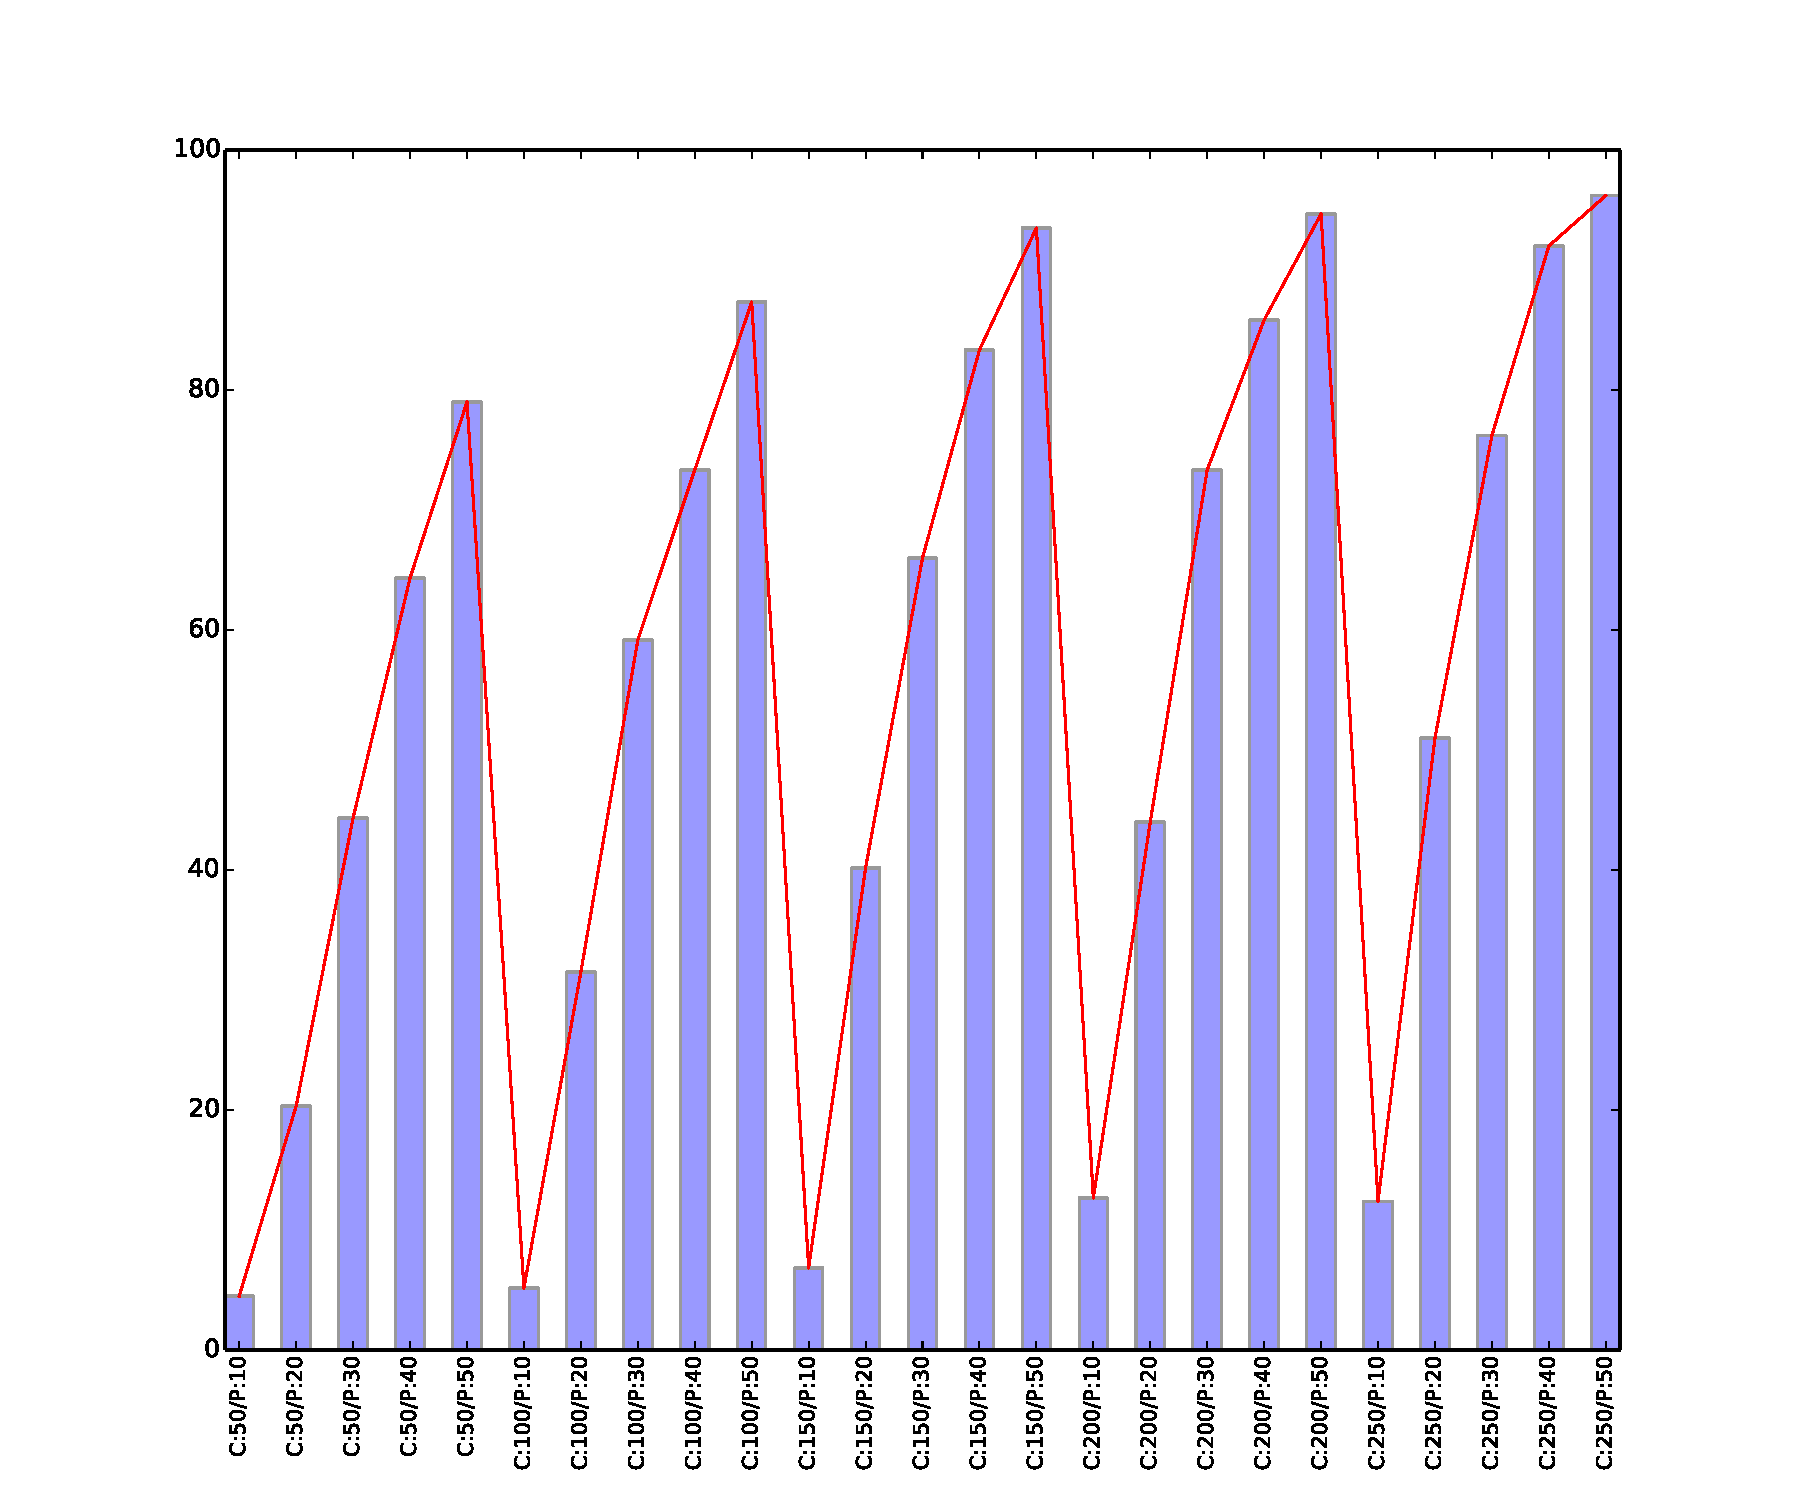
\includegraphics[width=0.8\textwidth]{images/C_G_div5_solved.pdf}
  \caption[Durch fünf teilbar Problem - \Gls{c_g_alg}]{Durch fünf teilbar Problem - \Gls{c_g_alg}}
  \label{fig:c_g_div5}
\end{figure}

Die Eingabeparameter für die Abbildung \ref{fig:c_g_div5} waren:
\begin{itemize}
	\item Problemmengengrösse: 10, 20, 30, 40, 50
	\item Populationsgrösse: 50, 100, 150, 250
\end{itemize}

In dieser Abbildung zeichnet sich ein \flqq Haifischzahn förmiges\frqq Muster ab, was darauf schliessen lässt, dass dieser Algorithmus mit zu kleinen Problemmengen sehr schlecht konvergiert. Dies kann auch nur teilweise durch die Verwendung von grösseren Populationen wettgemacht werden. Um dies weiter zu untersuchen wurden bei dieser Aufgabenstellung (\flqq durch fünf Teilbar Problem\frqq) Tests bei konstanter Populationsgrösse durchgeführt. 

\begin{figure}[ht]
  \centering
  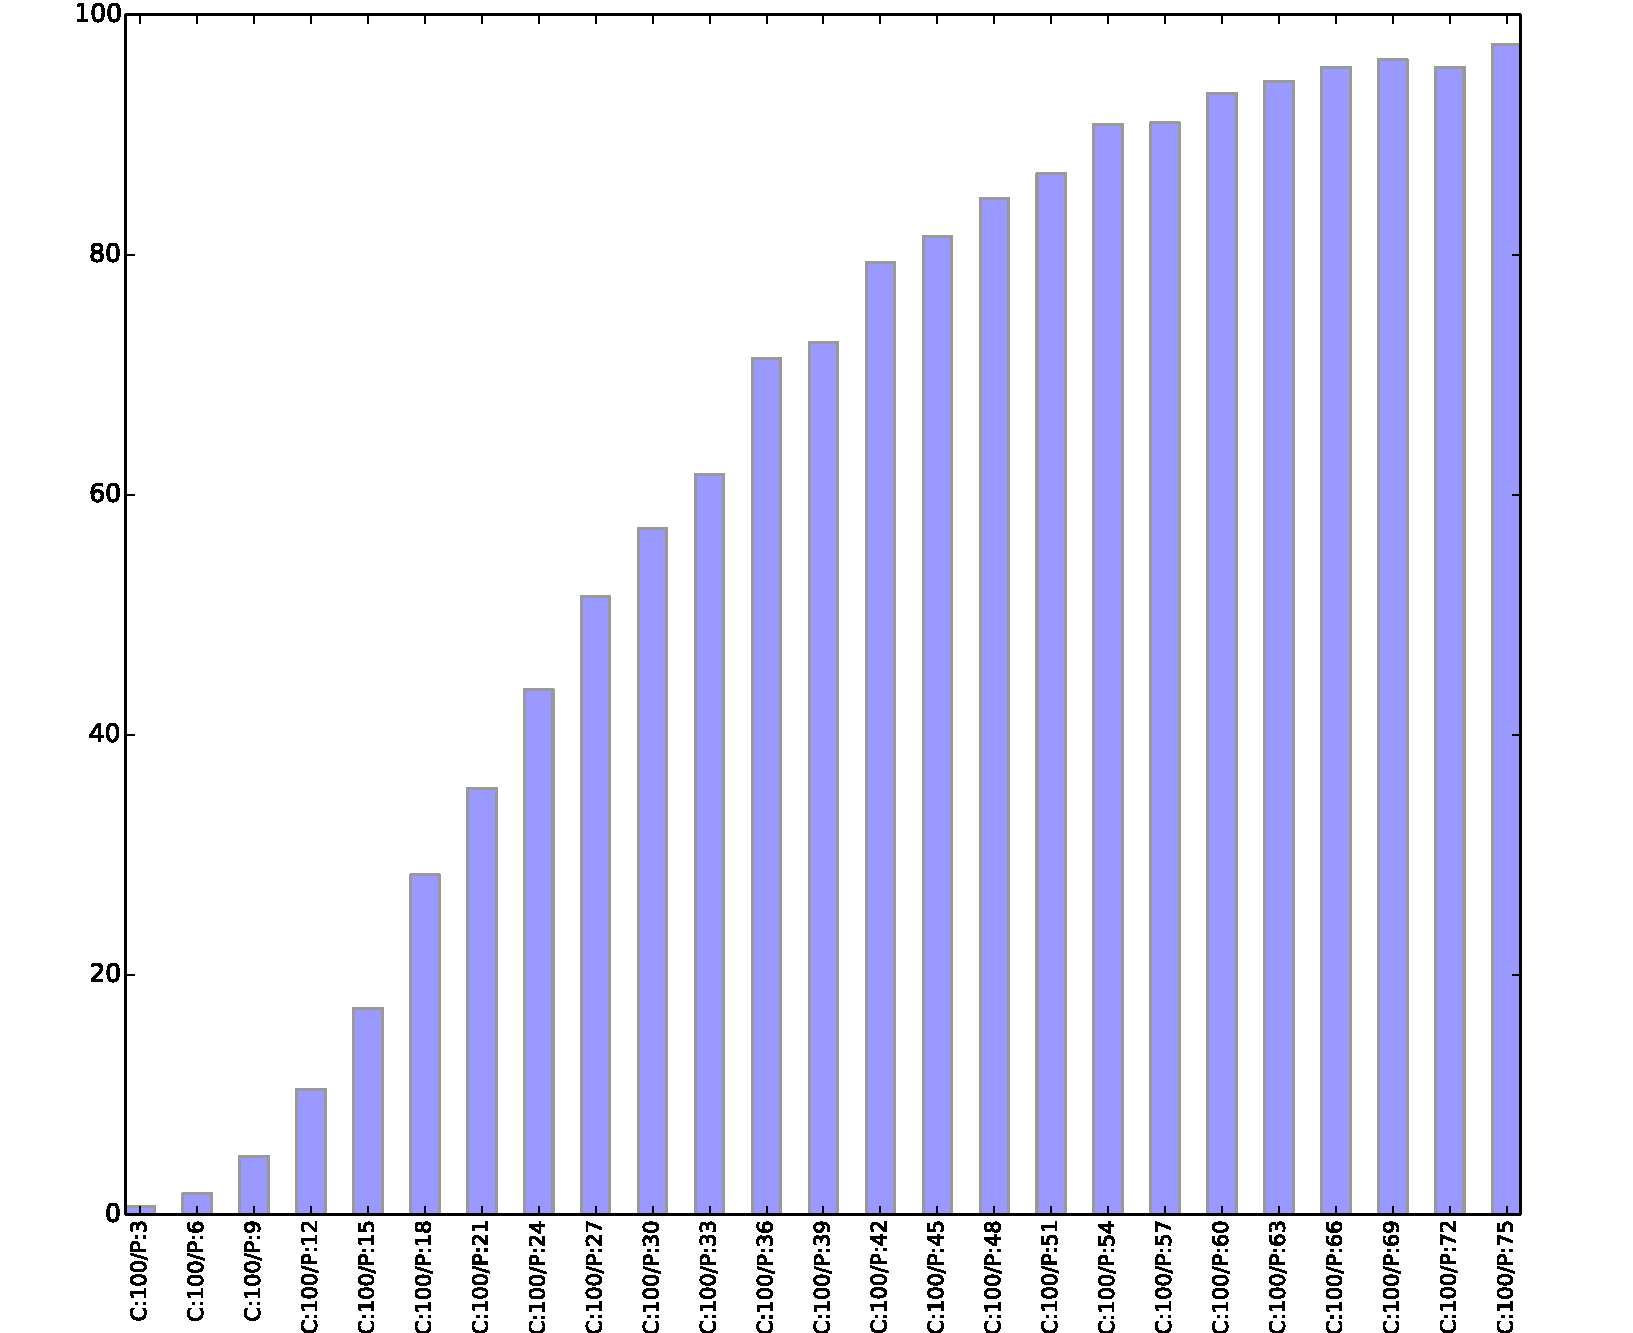
\includegraphics[width=0.78\textwidth]{images/C_G_PS_div5PS_solved.pdf}
  \caption[\Gls{c_g_alg} - Skalierung mit Problemmengengrösse]{\Gls{c_g_alg} - Skalierung mit Problemmengengrösse}
  \label{fig:c_g_ps_div5}
\end{figure}

\begin{figure}[H]
  \centering
  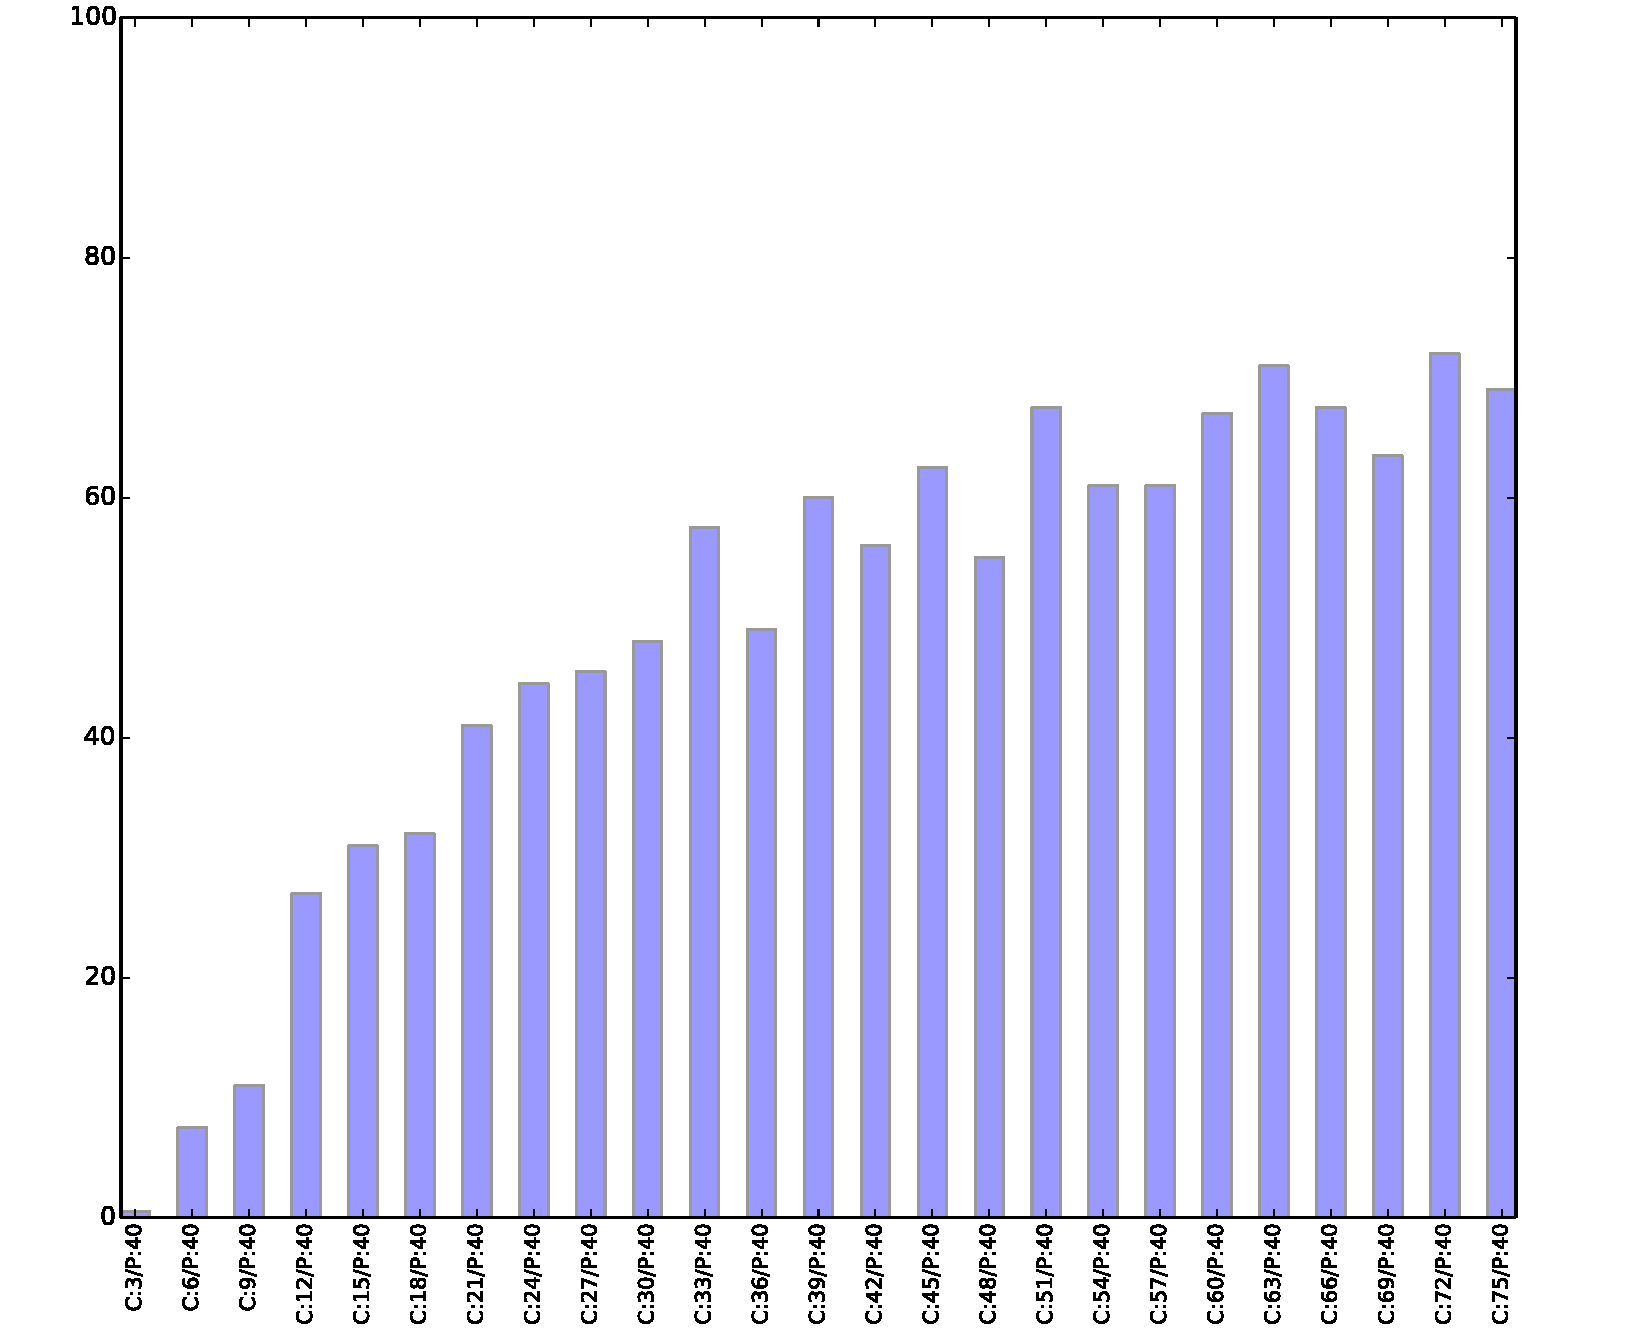
\includegraphics[width=0.78\textwidth]{images/C_G_CS_div5CS_solved.pdf}
  \caption[\Gls{c_g_alg} - Skalierung mit Populationsgrösse]{\Gls{c_g_alg} - Skalierung mit Populationsgrösse}
  \label{fig:c_g_cs_div5}
\end{figure}

Die Eingabeparameter für die Abbildung \ref{fig:c_g_ps_div5} waren:
\begin{itemize}
	\item Problemmengengrösse: 3, 6, 9, 12, ..., 72, 75
	\item Populationsgrösse: 100
\end{itemize}

In Abbildung \ref{fig:c_g_ps_div5} sieht man wie eine zu kleine Problemmenge den Erfolg des Algorithmus einschränken kann. Jedoch flacht die Kurve ab circa 40 Problemen langsam ab und ab circa 65 Problemen scheint eine Vergrösserung der Problemmenge zu keiner signifikanten Verbesserung des Ergebnisses mehr zu führen.


Um zu messen wie der Algorithmus mit der Populationsgrösse skaliert, wurde eine Testreihe mit fixer Anzahl Probleme und variabler Populationsgrösse implementiert.

Die Eingabeparameter für die Abbildung \ref{fig:c_g_cs_div5} waren:
\begin{itemize}
	\item Problemmengengrösse: 40
	\item Populationsgrösse: 3, 6, 9, 12, ..., 72, 75
\end{itemize}

Hier wurde bewusst eine zu kleine Problemmenge gewählt um nicht an die 100\% Marke zu kommen. Man sieht hier wiederum, dass der Algorithmus mit sehr kleinen Mengen ($3$, $6$, $9$ Individuen) praktisch gar nicht konvergiert. Die Kurve steigt danach steil an und flacht ab einer Populationsgrösse von circa 35 ab, steigt jedoch weiter.